\chapter{Deployment \& Component Diagrams}

\section*{E.1 Deployment Diagram}\label{fig:deploy_diagram}

\begin{figure}[H]
\centering
\begin{tikzpicture}[
  node/.style={rectangle, draw=cuetblue, fill=cuetblue!8, rounded corners,
               minimum width=3cm, minimum height=1cm, font=\small, align=center},
  device/.style={rectangle, draw=cuetgold, fill=cuetgold!8,
                 minimum width=3.5cm, minimum height=1.4cm, font=\small\bfseries, align=center},
  arrow/.style={-Stealth, thick, color=cuetblue},
  dashed_arr/.style={-Stealth, thick, dashed, color=gray}
]
  % Devices
  \node[device] (phone)   at (0,8)   {Android / Web\\(Flutter Client)};
  \node[device] (server)  at (6,8)   {Ubuntu 22.04 LTS\\(Docker Host)};
  \node[device] (target)  at (12,8)  {Linux Server\\(Monitored Host)};
  \node[device] (google)  at (12,4)  {Google Cloud\\(Gemini API)};
  \node[device] (firebase) at (0,4)  {Firebase\\(FCM Push)};

  % Backend services
  \node[node] (nginx)    at (6,6.5)  {Nginx\\(HTTPS proxy)};
  \node[node] (django)   at (4.5,5)  {Django\\(Daphne ASGI)};
  \node[node] (celery)   at (7.5,5)  {Celery\\Worker/Beat};
  \node[node] (redis)    at (6,3.5)  {Redis};
  \node[node] (postgres) at (4,2)    {PostgreSQL 18};
  \node[node] (mlsvc)    at (8,2)    {FastAPI\\ML Service};
  \node[node] (vms)      at (6,0.5)  {VictoriaMetrics\\Cluster (3 nodes)};
  \node[node] (alloy)    at (12,6)   {Grafana\\Alloy Agent};

  % Connections
  \draw[arrow] (phone) -- node[font=\scriptsize,above]{HTTPS/WSS} (nginx);
  \draw[arrow] (nginx) -- (django);
  \draw[arrow] (django) -- (redis);
  \draw[arrow] (celery) -- (redis);
  \draw[arrow] (django) -- (postgres);
  \draw[arrow] (celery) -- (postgres);
  \draw[arrow] (celery) -- node[font=\scriptsize]{classify} (mlsvc);
  \draw[arrow] (mlsvc) -- (vms);
  \draw[arrow] (django) -- node[font=\scriptsize]{query} (vms);
  \draw[dashed_arr] (django) -- (google);
  \draw[dashed_arr] (celery) -- (google);
  \draw[dashed_arr] (django) -- (firebase);
  \draw[arrow] (target) -- (alloy);
  \draw[arrow] (alloy) -- node[font=\scriptsize]{remote-write} (django);
\end{tikzpicture}
\caption{Deployment diagram for Infra Monitor (Docker Compose on Ubuntu 22.04)}\label{fig:deploy}
\end{figure}

\section*{E.2 Data Flow Diagrams (DFD)}

The following DFDs are from \texttt{report/diagrams/new\_dfds/} and show
the data flows at multiple levels of abstraction.

\begin{figure}[H]
\centering
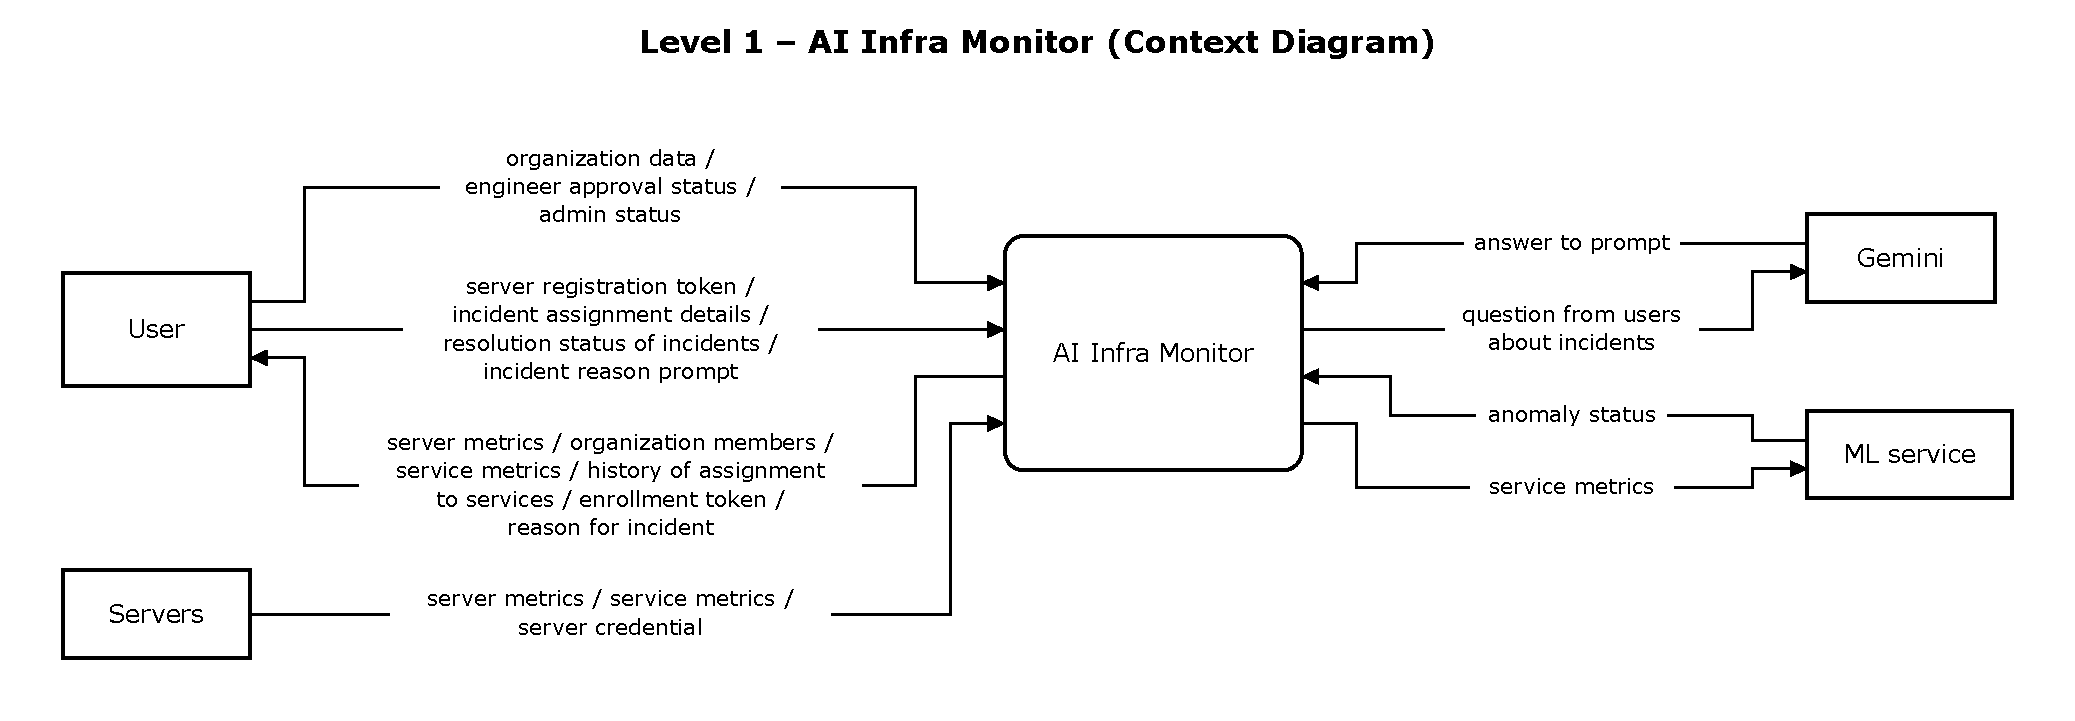
\includegraphics[width=0.92\textwidth]{01_level1_context.pdf}
\caption{DFD Level 1: Context diagram -- Infra Monitor as a black box}\label{fig:dfd1}
\end{figure}

\begin{figure}[H]
\centering
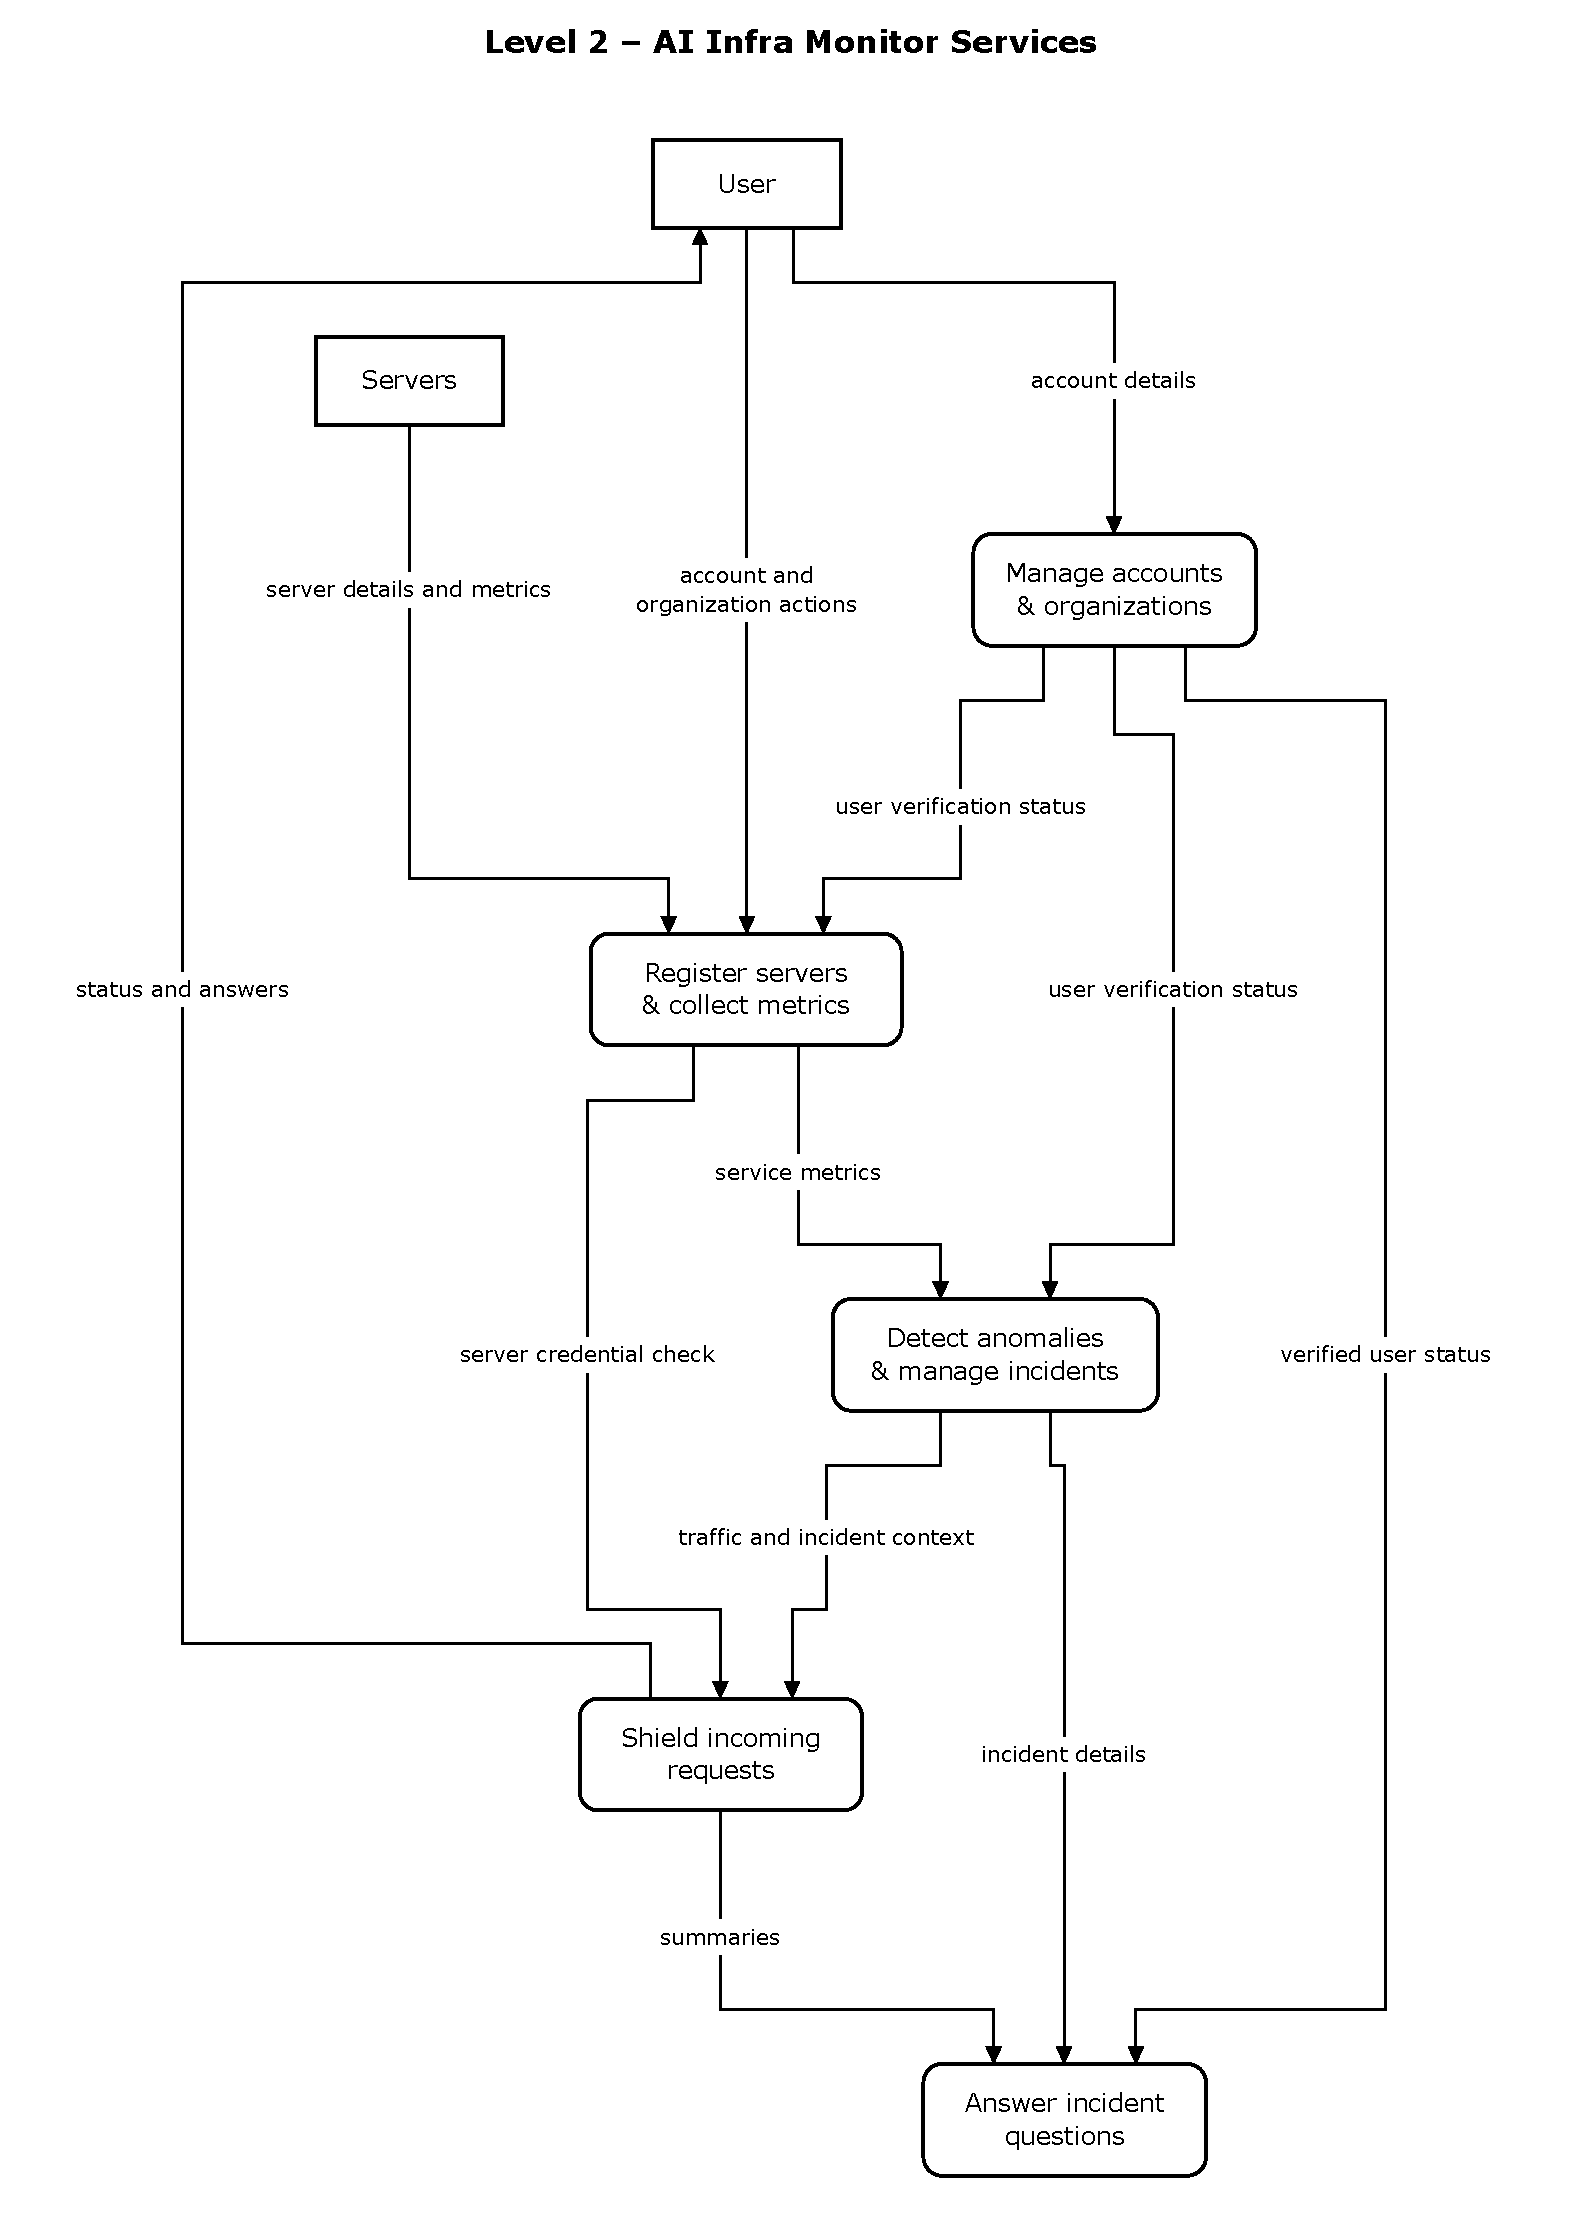
\includegraphics[width=0.92\textwidth]{02_level2_services.pdf}
\caption{DFD Level 2: Service decomposition}\label{fig:dfd2}
\end{figure}

\begin{figure}[H]
\centering
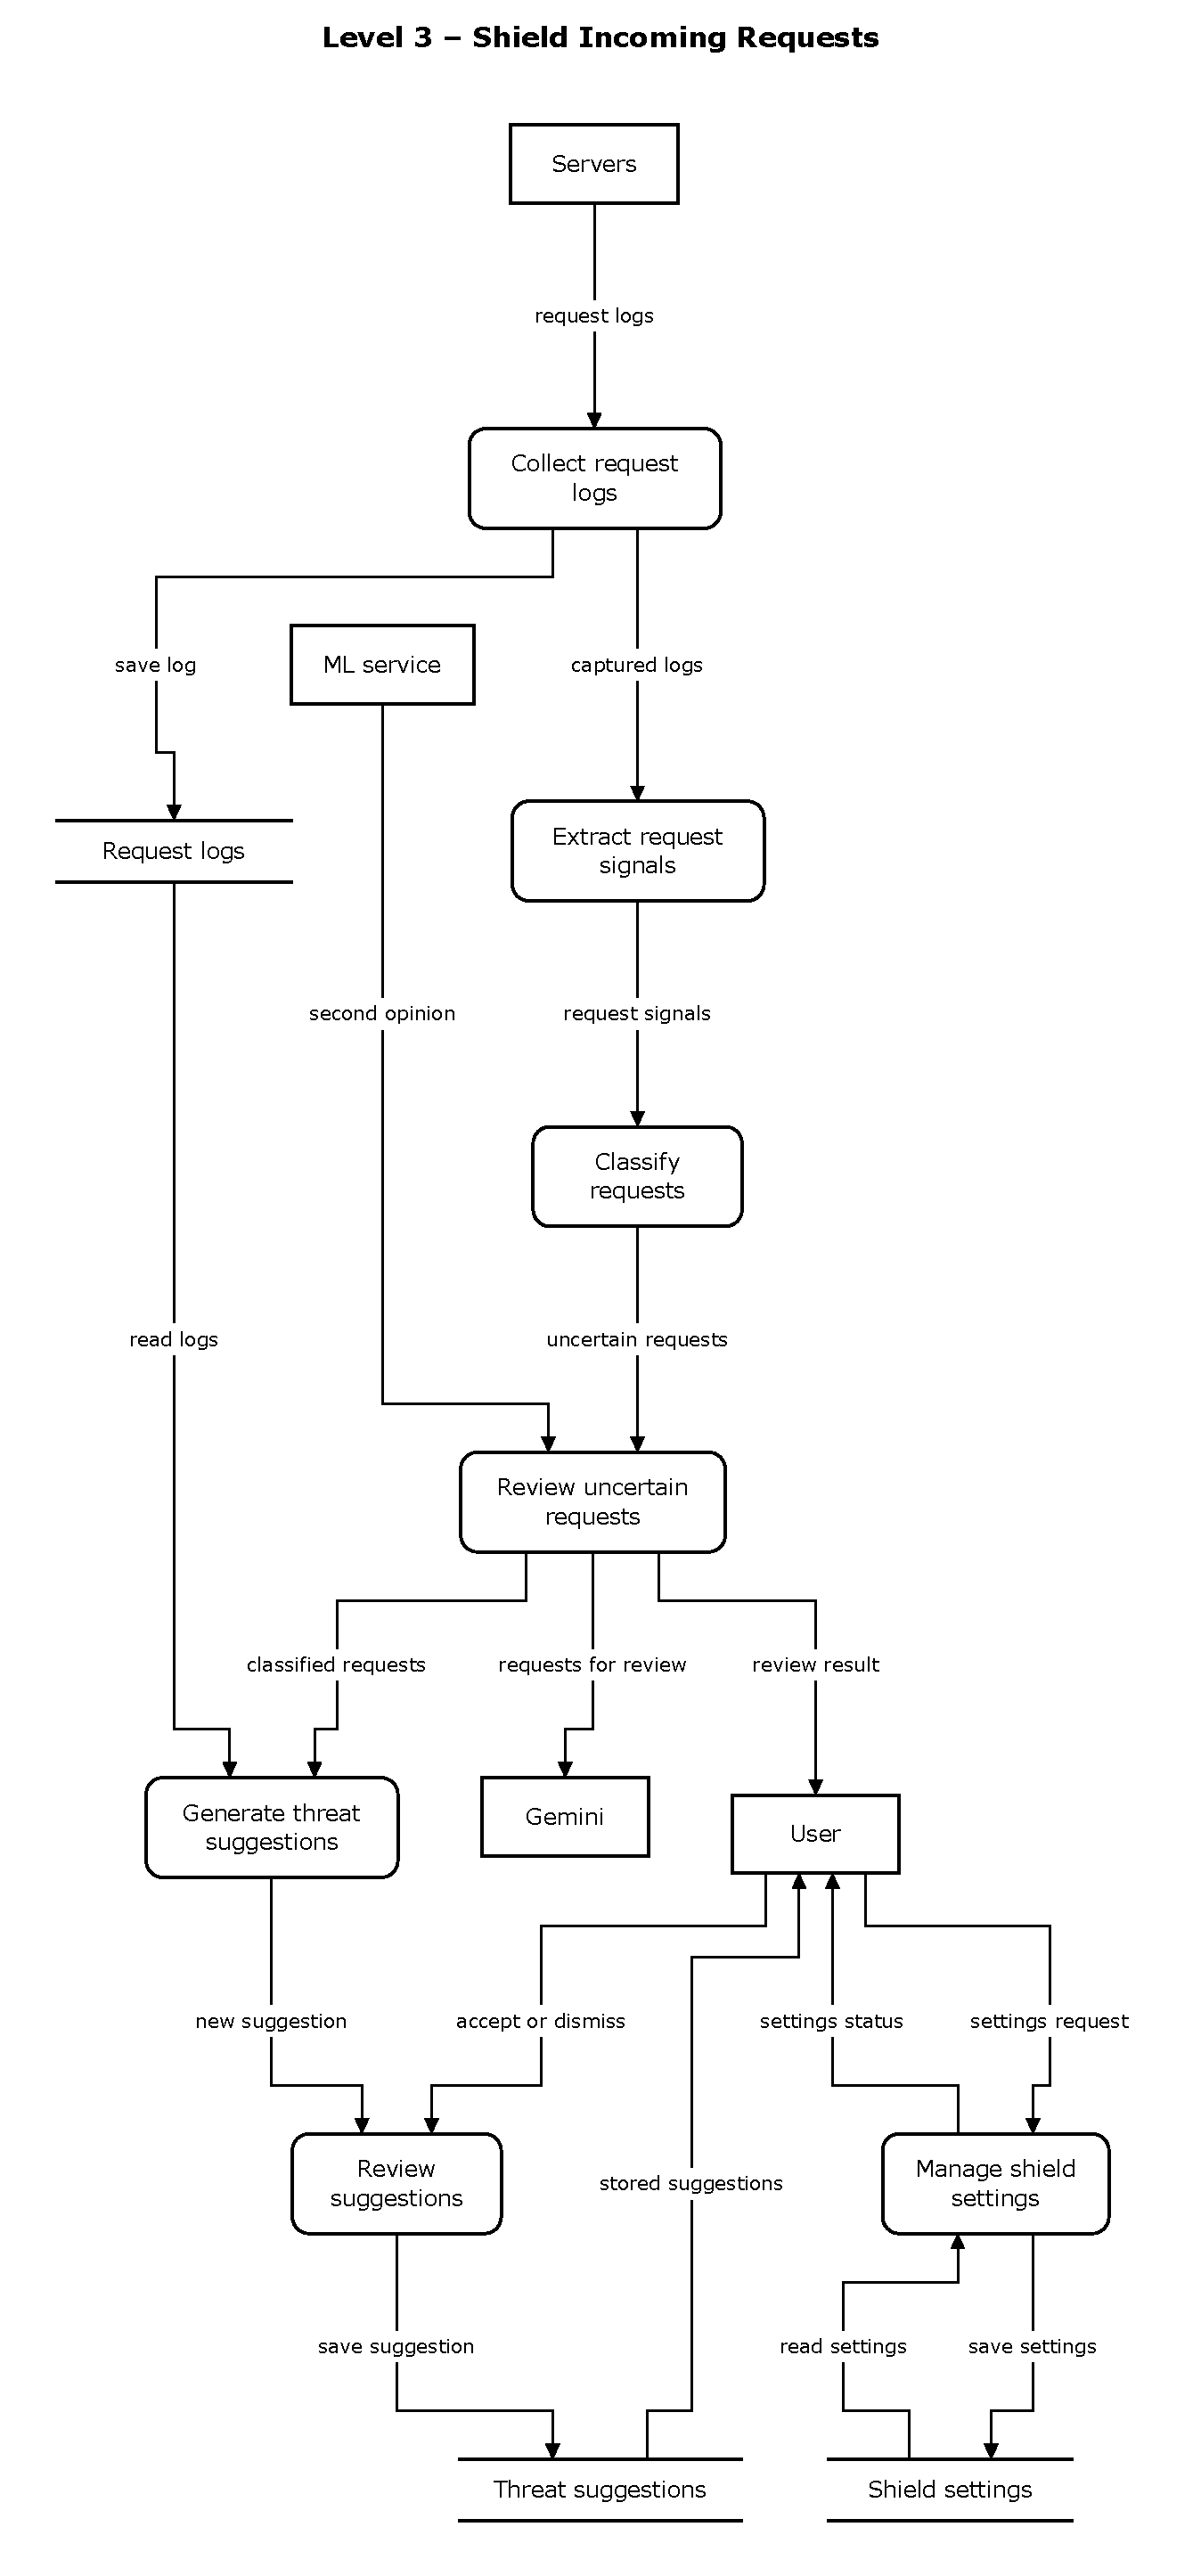
\includegraphics[width=0.92\textwidth]{03_level3_shield.pdf}
\caption{DFD Level 3: Request Shield internal data flows}\label{fig:dfd3}
\end{figure}

\begin{figure}[H]
\centering
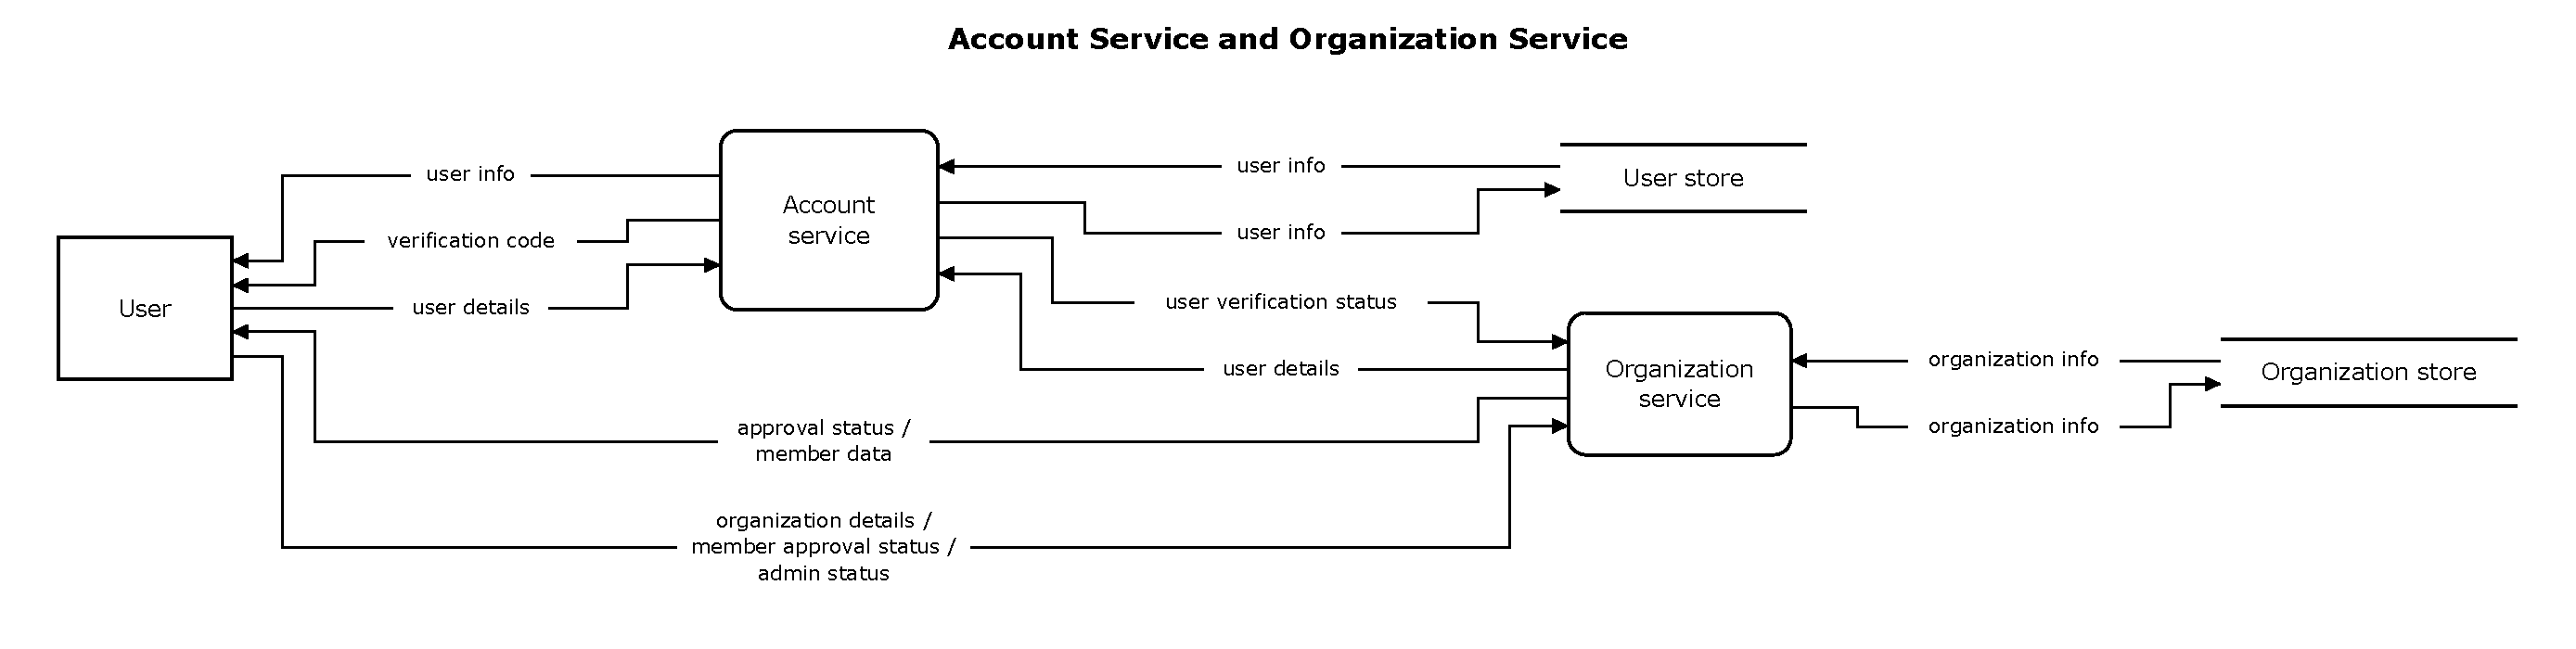
\includegraphics[width=0.92\textwidth]{04_account_organization.pdf}
\caption{DFD: Account and Organisation flows}\label{fig:dfd4}
\end{figure}

\begin{figure}[H]
\centering
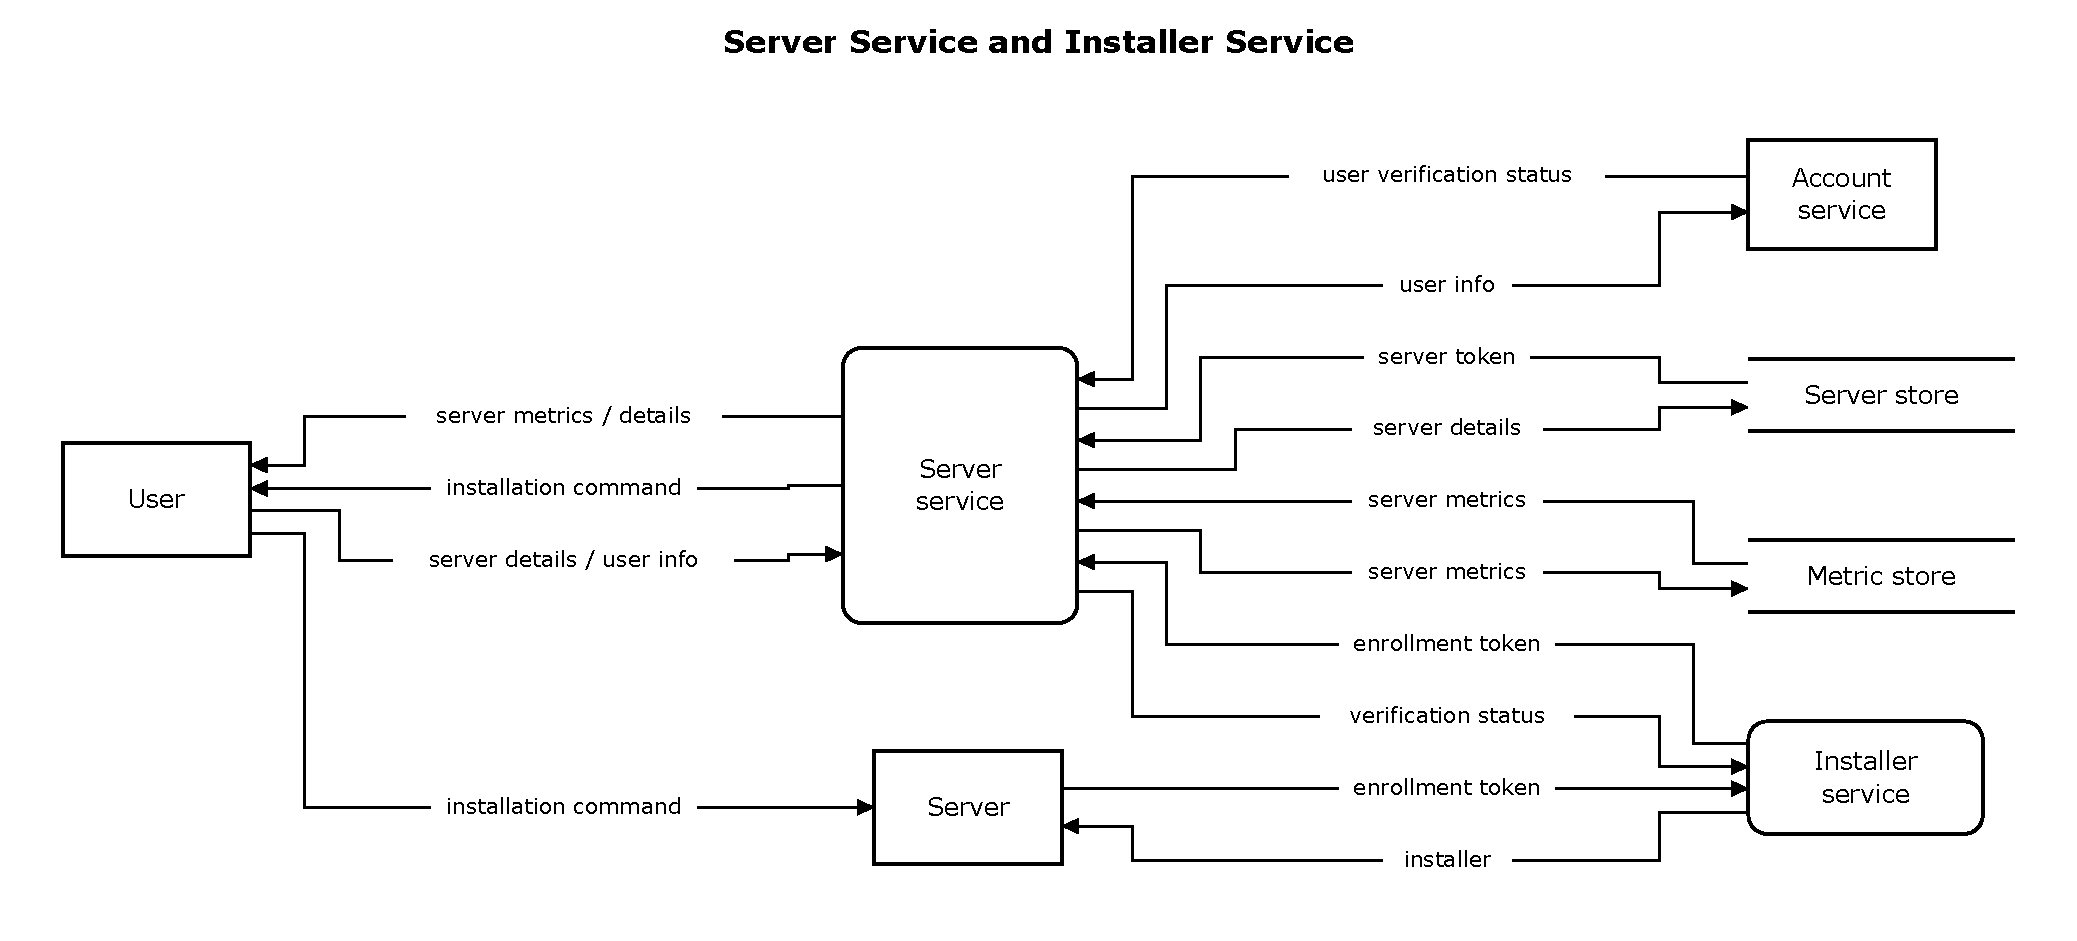
\includegraphics[width=0.92\textwidth]{05_server_installer.pdf}
\caption{DFD: Server installer and enrollment flows}\label{fig:dfd5}
\end{figure}

\begin{figure}[H]
\centering
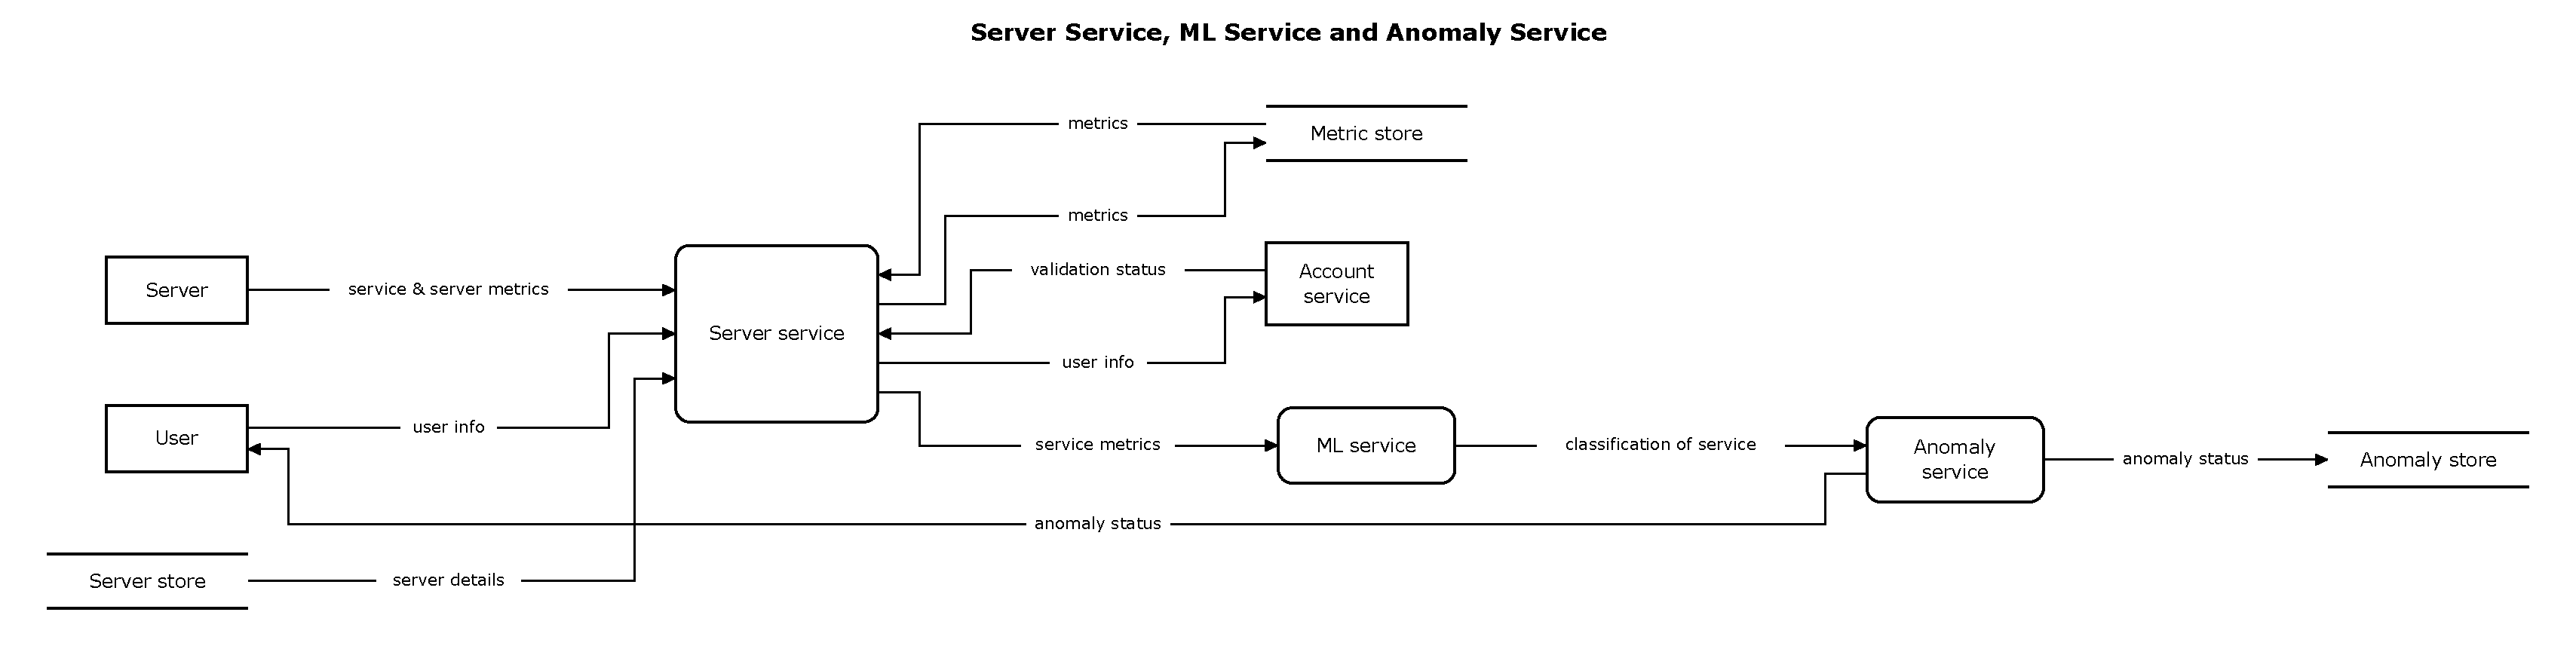
\includegraphics[width=0.92\textwidth]{06_server_ml_anomaly.pdf}
\caption{DFD: Server metric collection and ML anomaly detection}\label{fig:dfd6}
\end{figure}

\begin{figure}[H]
\centering
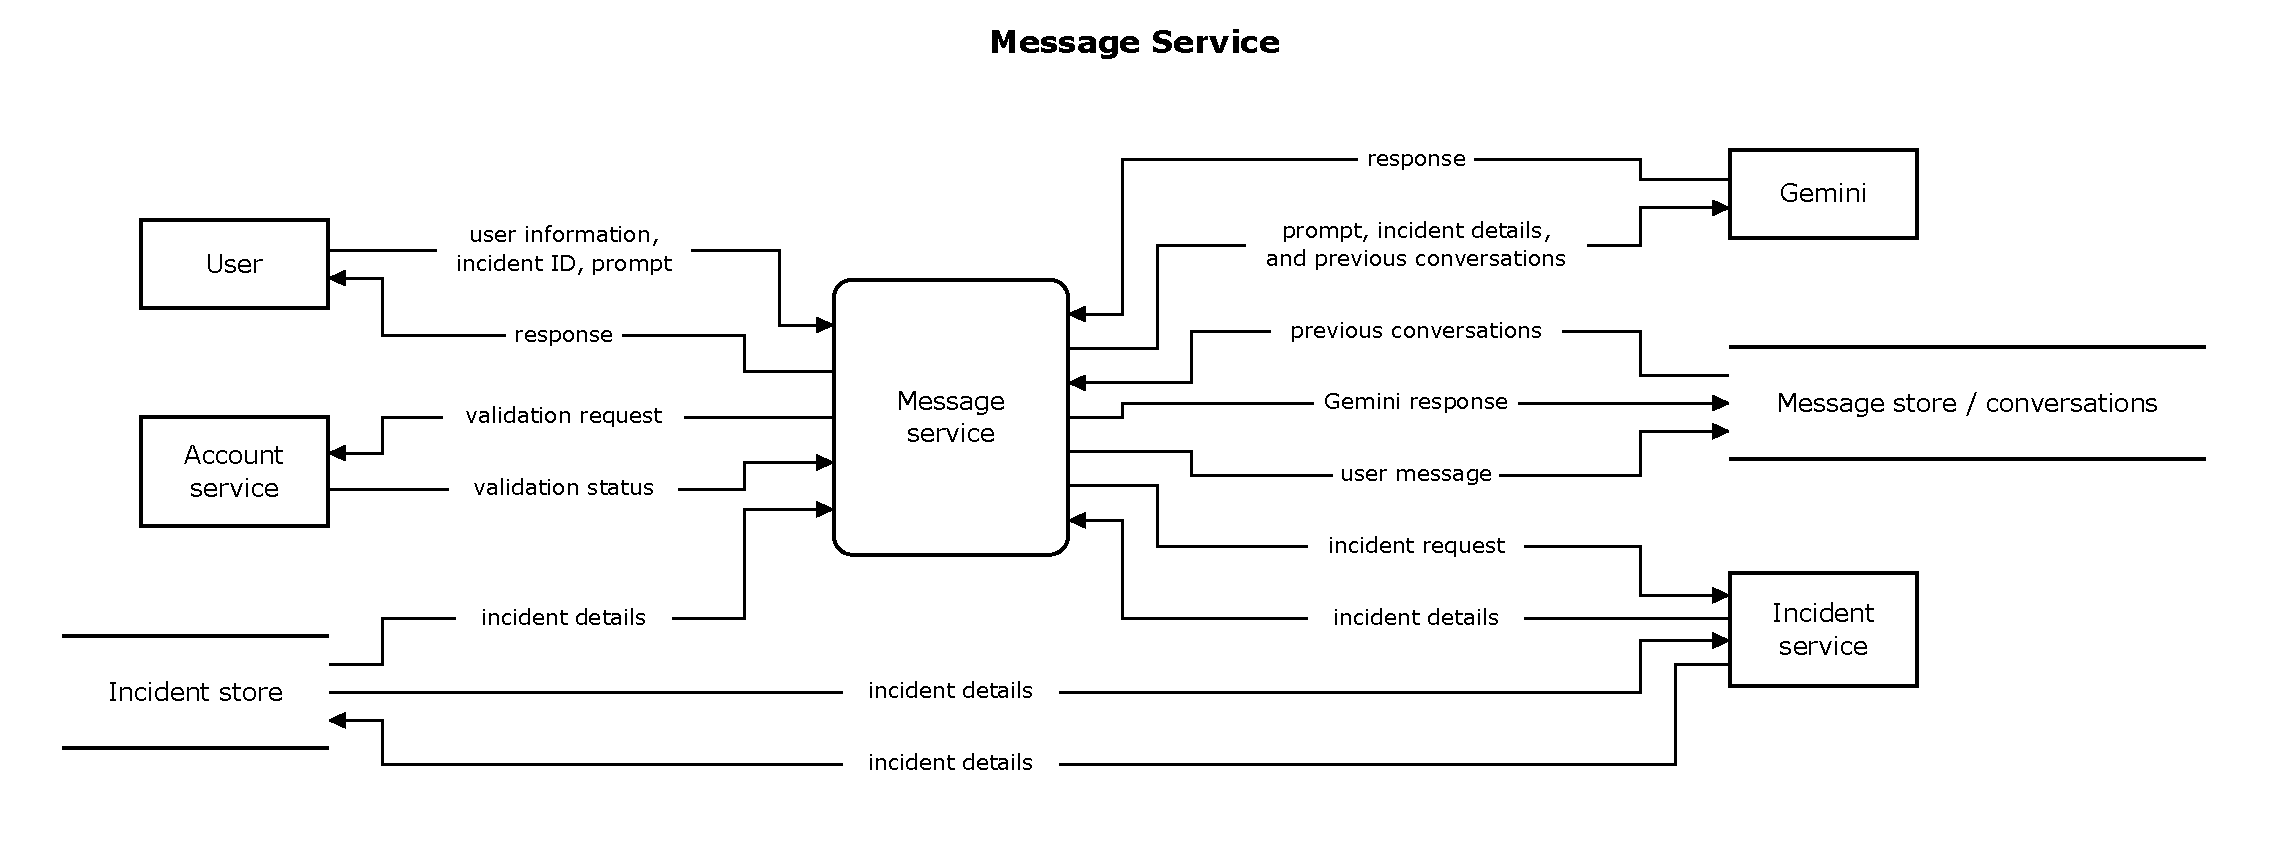
\includegraphics[width=0.92\textwidth]{07_message_service.pdf}
\caption{DFD: Message / notification service flows}\label{fig:dfd7}
\end{figure}

